% ================= CHAPTER 2 =================
\chapter{LITERATURE REVIEW}

\section{Line Spacing}
The line spacing from the chapter title to the sub-chapter is 3 lines. The distance from the sub-chapter to the first sentence is 1.5 lines.

\subsection{Sub-sub Chapter}
If a sub-sub chapter is required, it is typed using an underline but not in bold. The numbering follows the sub-chapter such as 2.1.1; 2.1.2; 2.1.3; etc.

\subsection{Sub-sub Chapter}
Example of other sub-sub chapter usage.

\section{Equations}
Equations are written using the equation feature in LaTeX. An example of writing an equation can be seen in equation \ref{eq:rho}.

\begin{equation}
    \rho = \frac{m}{V}
    \label{eq:rho}
\end{equation}

\section{Figures}
Figures can be in the form of photos or graphs/schemes needed in research and show a relationship with the research content. The titles of figures and graphs are placed below the object with numbering adjusted to the chapter. Figure titles that only require 1 line are typed in centered format. If the figure title requires more than one line, the title is typed with 1 spacing in justify format, the second or more lines adjust the indentation of the first letter of the figure title. Bold is used for writing figure titles. Because the figure title is a sentence, it ends with a period. Generally, figures are placed at the beginning of the page or at the end of the page.

\begin{figure}[htbp]
    \centering
    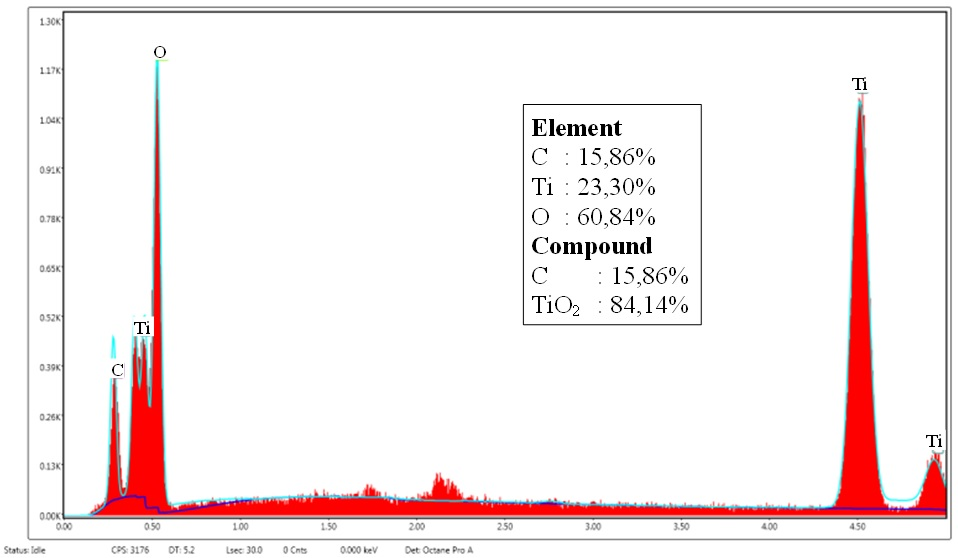
\includegraphics[width=0.6\textwidth]{assets/images/gambar_1}
    \caption{EDS spectrum of the PP surface coated with TiO$_2$.}
    \label{fig:eds}
\end{figure}

If a figure is referred to in the narrative, the first letter of the word 'Figure' is written with a capital letter (Figure \ref{fig:eds}; Figure \ref{fig:deposisi}; Figure 4.3; and so on) even if it is in the middle of a sentence. An example of presenting a figure title that requires 1 line can be seen in Figure \ref{fig:eds}. The way to write a figure title that requires more than 1 line is presented in Figure \ref{fig:deposisi}.

\begin{figure}[htbp]
    \centering
    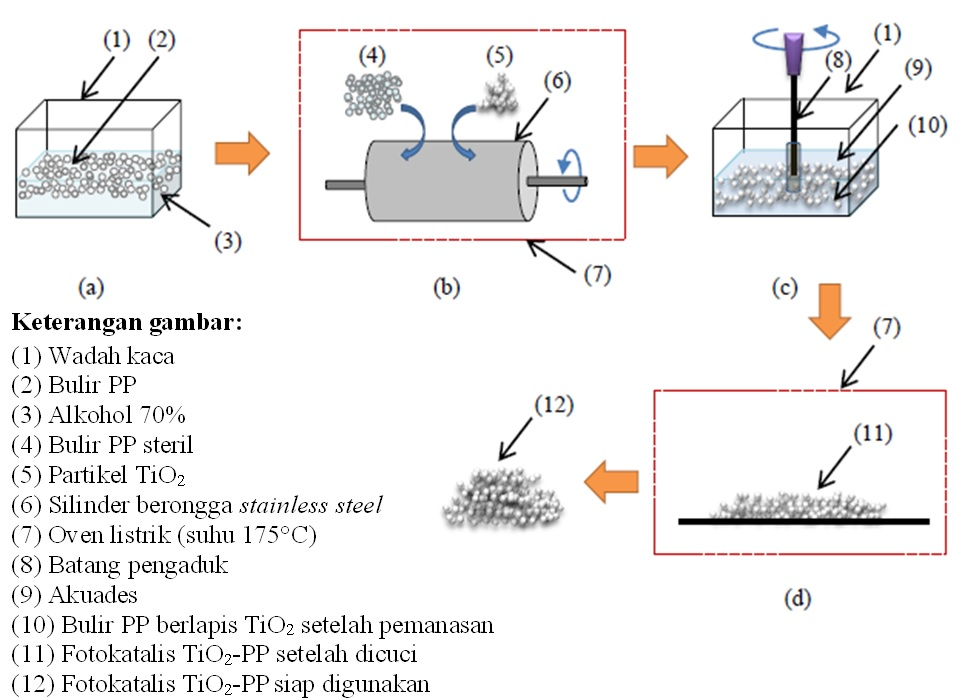
\includegraphics[width=0.6\textwidth]{assets/images/gambar_2}
    \caption{Deposition of TiO$_2$ on the PP surface was carried out by (a) cleaning the PP beads using 70\% alcohol, (b) immobilizing TiO$_2$ on the PP surface with the thermal milling method to produce TiO$_2$-PP, (c) cleaning TiO$_2$-PP, and (d) drying the resulting photocatalyst.}
    \label{fig:deposisi}
\end{figure}

\section{Tables}
Tables are made with horizontal lines only without vertical lines. The font size in the table is allowed to be less than 12 as long as the writing is still clearly legible. The table title is placed above the object with numbering adjusted to the chapter. Similar to figure titles, if the table title only requires 1 line, it is typed in centered format. If the table title requires more than one line, the title is typed with 1 spacing in justify format, the second or more lines adjust the indentation of the first letter of the table title. Unlike bold for writing figure titles, the table title is not in bold.

\begin{table}[htbp]
    \centering
    \caption{Thermal milling deposition rate for time variations.}
    \begin{tabular}{ccc}
        \toprule
        Milling time (minutes) & Mass of deposited TiO$_2$ (g) & Deposition rate (mg/s) \\
        \midrule
        0 & 0 & 0.06 \\
        20 & 0.6 & 1.05 \\
        25 & 0.9 & 0.95 \\
        30 & 1.1 & 0.31 \\
        \bottomrule
    \end{tabular}
    \label{tab:milling}
\end{table}

If a table is referred to in the narrative, the first letter of the word 'Table' is written with a capital letter (Table \ref{tab:milling}; Table \ref{tab:absorbansi}; Table 4.3; etc.) even if it is in the middle of a sentence. An example of presenting a table title that requires 1 line can be seen in Table \ref{tab:milling}. The way to write a table title that requires more than 1 line is presented in Table \ref{tab:absorbansi}.

\begin{table}[htbp]
    \centering
    \caption{Average absorbance value ($A$) as a function of time for each repetition of TiO$_2$-PP use.}
    \begin{tabular}{ccccccc}
        \toprule
        Use No. & \multicolumn{6}{c}{Average value of $A$ every 8 hours (a.u)} \\
        \cmidrule(lr){2-7}
        & 0 hours & 8 hours & 16 hours & 24 hours & 32 hours & 40 hours \\
        \midrule
        1 & 2.89 & 1.637 & 1.217 & 1.130 & 0.154 & 0.154 \\
        2 & 2.89 & 1.559 & 1.522 & 0.546 & 0.186 & 0.15 \\
        3 & 2.89 & 1.645 & 1.272 & 0.630 & 0.154 & 0.156 \\
        4 & 2.89 & 1.602 & 1.340 & 1.326 & 0.225 & 0.206 \\
        5 & 2.89 & 1.644 & 1.586 & 1.400 & 0.916 & 0.465 \\
        \bottomrule
    \end{tabular}
    \label{tab:absorbansi}
\end{table}
